\documentclass[11pt]{article}
\usepackage[margin=1in]{geometry}
\usepackage{amsmath,amssymb}
\usepackage{graphicx}
\usepackage[hidelinks]{hyperref}
\usepackage{natbib}
\setcitestyle{numbers,square}

\title{\textbf{The Geometry of Gravitational-Wave Inference:\\
reconstructing component-mass posterior orientation from the chirp-mass curve}}
\author{Kunal Bhatia\\
\small Independent researcher, Meerut, India \\
\small ORCID: 0009-0007-4447-6325}
\date{Draft --- \today}

% AUTO-GENERATED by src/build_manuscript_figures.py -- do not edit by hand.
% Every number below is read from a figure sidecar JSON, so captions cannot drift from the figures.
%
% Captions state what is plotted and the takeaway. Provenance, selection rules and methodological
% caveats belong in the text -- an external readability review flagged the earlier captions as
% mini-methods sections.

\newcommand{\figonebcaption}{%
Reconstruction error against the local linear approximation, on elongated events
($\mathrm{axr}\ge3$) in three disjoint catalogs. Each thin line is one event, joining
its median-point tangent error to its constant-$\mathcal{M}_c$ curve error; heavy bars are catalog
medians with a bootstrap interval over events. The curve improves on the tangent in every catalog:
GWTC-3 ($n=29$): $4.83^\circ \to 0.88^\circ$, O4a ($n=19$): $6.67^\circ \to 1.26^\circ$, O4b ($n=32$): $4.20^\circ \to 1.19^\circ$. Note the logarithmic scale.}

\newcommand{\figoneccaption}{%
The reconstruction requires the \emph{event's own} mass-ratio marginal. Blue circles use the event's own
$q$ marginal, orange squares the median-point tangent, grey diamonds a $q$ marginal pooled over the
catalog. The grey band spans the 5th--95th percentile of a permutation null in which each event is given a
different event's $q$ marginal (300 catalog-stratified draws); the
dark tick marks that null's minimum. Own-$q$ falls below the null minimum in every catalog (GWTC-3: own-$q$ $0.88^\circ$ vs.\ null minimum $4.55^\circ$; O4a: own-$q$ $1.26^\circ$ vs.\ null minimum $3.19^\circ$; O4b: own-$q$ $1.19^\circ$ vs.\ null minimum $2.23^\circ$).}

\newcommand{\figtwoacaption}{%
Posterior geometry for three events chosen by fixed rules --- \emph{clean success (high elongation)} GW241011\_233834 (O4b, axr $29.3$, curve $0.08^\circ$, tangent $0.91^\circ$); \emph{typical} GW190728\_064510 (GWTC-3, axr $6.0$, curve $1.04^\circ$, tangent $13.97^\circ$); \emph{worst case} GW200308\_173609 (GWTC-3, axr $4.5$, curve $16.32^\circ$, tangent $23.61^\circ$). Each panel shows the posterior
samples, the constant-$\mathcal{M}_c$ curve, the measured principal axis and the two predicted
orientations, on equal-aspect axes. The worst case is included by rule rather than chosen, and carries a
zoom inset on its dense core; its failure is genuine, the error remaining at
$16.2$--$17.5^\circ$ when the sample is trimmed to its central $90\%$. Across all
elongated events the tangent beats the curve for
$15\%$ of events, rising to
$31\%$ above $\mathrm{axr}=8$.}


\begin{document}
\maketitle

\begin{abstract}
The parameter-estimation posteriors of compact-binary gravitational-wave events have a shape that is
usually treated as a nuisance. We show instead that this shape is highly structured: the principal-axis
orientation of each source-frame $(m_1,m_2)$ posterior can be \emph{reconstructed} from two one-dimensional
summaries of that same posterior --- its median chirp mass and its mass-ratio marginal --- using the
constant-chirp-mass curve and \emph{no coefficients calibrated on the validation catalogs}. This is a
posterior-compression result, not a prediction from source medians alone: the $q$ marginal is an input taken
from the posterior being reconstructed, and we quantify how much of the accuracy it supplies. Derived on
GWTC-3 and locked before opening later data, the reconstruction reaches a median mismatch of $1.26^\circ$
(GWTC-4.0/O4a) and $1.22^\circ$ (GWTC-5.0/O4b) on elongated events, against $5$--$7^\circ$ for the local
tangent approximation that underlies rapid parameter-estimation tools. The result is not the trivial
statement that a curve fits a curved posterior: substituting any other event's mass-ratio marginal degrades
it by $2.5$--$12\times$, and the achieved error lies below the \emph{minimum} of $300$ catalog-stratified
permutations in every catalog. It also transfers across waveform families --- inputs from one family
recover a different family's separately inferred axis to $2.1^\circ$, against a $2.0^\circ$ reference scale
set by how much those families disagree with each other --- so it is not an artifact of reusing one
posterior's sampling noise. The residual $\sim\!1^\circ$ is \emph{not} sampling noise but a real
systematic, roughly six times the Monte Carlo resolution of the released samples; finite posterior
thickness, which the zero-thickness curve model omits by construction, is supported out-of-sample as a
contributor, while arc-varying thickness is not established. We report the result as a reconstruction law
and a diagnostic, and explicitly not as a test of general relativity: the posteriors were produced with
general-relativistic waveform models, so their internal geometry cannot bound deviations from it.
\end{abstract}

\section{Introduction}
Gravitational-wave (GW) parameter estimation delivers, for each detected compact-binary coalescence, a
posterior probability distribution over the source parameters. It is a commonplace that the chirp mass
$\mathcal{M}_c = (m_1 m_2)^{3/5}/(m_1+m_2)^{1/5}$ is the best-measured mass combination and that the
component-mass posterior forms an elongated ``banana'' lying along near-constant-$\mathcal{M}_c$ contours
\citep{CutlerFlanagan1994,PoissonWill1995,Hannam2013}. This paper asks a sharper question: is the
\emph{geometry} of that posterior --- specifically the orientation of its principal axis --- quantitatively
\emph{reconstructible}, event by event, from a small number of one-dimensional summaries with no
coefficients calibrated on the validation data, and does the reconstruction survive out-of-sample on
later, disjoint event catalogs?

We answer yes. The organizing thesis is that the uncertainty geometry of GW inference is \emph{measurement
optics}: it is a property of what the instrument and signal can and cannot resolve, largely independent of
source astrophysics. This viewpoint is not new mathematically --- it is the content of the
``sloppy model'' framework \citep{Transtrum2015} and of principal curves \citep{HastieStuetzle1989}. Our contribution is to make it quantitative and validated
out-of-sample for GW posteriors, and to use it as a systematics diagnostic. We do \emph{not} present it as
a test of general relativity; Sec.~\ref{sec:gr} explains why the geometry of GR-generated posteriors cannot
serve that purpose.

\section{The curved chirp-mass law}
\subsection{Definition}
For an event with source-frame samples $\{(m_1,m_2)\}$, let $\psi_{\rm meas}$ be the position angle of the
principal axis of the sample covariance, and let the axis ratio $\mathrm{axr}$ be the ratio of its
principal standard deviations. The constant-$\mathcal{M}_c$ \emph{curve} through the plane is
\begin{equation}
m_1(q) = \mathcal{M}_c\,(1+q)^{1/5} q^{-3/5}, \qquad m_2 = q\,m_1,
\end{equation}
where $q=m_2/m_1\in(0,1]$ and $\mathcal{M}_c$ is the event's median source-frame chirp mass. The predicted
orientation $\psi_{\rm curve}$ is the principal axis of this curve evaluated over the event's own $q$
marginal. The local linear approximation $\psi_{\rm tangent}$ is the tangent to the contour at the median
point. No coefficient is calibrated on the validation catalogs: every ingredient is supplied by the event
itself.

It is important to be precise about what this is. The $q$ marginal is an input drawn from the very
posterior whose orientation is being reconstructed, so this is a \emph{compression} statement --- a
two-dimensional posterior's orientation recovered from one scalar and one one-dimensional marginal, using
no information from the $(m_1,m_2)$ covariance --- and not a prediction of posterior shape from source
medians or from physics external to the posterior. Sec.~\ref{sec:nontrivial} quantifies how much of the
accuracy that marginal supplies.

\subsection{Out-of-sample validation across three catalogs}
The law was derived from GWTC-1/2.1/3 events and its prediction placed on record before any later-catalog
file was opened. Table~\ref{tab:curve} reports the locked decision on two subsequent, disjoint catalogs.
On elongated events ($\mathrm{axr}\ge 3$, where orientation is well defined) the median mismatch
$|\psi_{\rm curve}-\psi_{\rm meas}|$ is $1.26^\circ$ (GWTC-4.0/O4a) and $1.22^\circ$ (GWTC-5.0/O4b); the
curve beats the tangent on the full catalogs, and the tangent-law replication statistics reproduce the
training-set values. The catalogs are mutually disjoint (zero shared events).

\begin{table}[h]
\centering
\begin{tabular}{lccc}
\hline
 & GWTC-3 (train) & GWTC-4.0/O4a & GWTC-5.0/O4b \\
\hline
median $|\psi_{\rm curve}-\psi_{\rm meas}|$ (elongated) & --- & $\mathbf{1.26^\circ}$ & $\mathbf{1.22^\circ}$ \\
median $|\psi_{\rm curve}-\psi_{\rm meas}|$ (all) & --- & $7.53^\circ$ & $5.41^\circ$ \\
median $|\psi_{\rm tangent}-\psi_{\rm meas}|$ (all) & $7.49^\circ$ & $9.36^\circ$ & $8.23^\circ$ \\
chirp-vs-total win fraction & $81\%$ & $86\%$ & $88\%$ \\
Spearman$(|\Delta\psi_{\rm tangent}|,\mathrm{axr})$ & $-0.42$ & $-0.40$ & $-0.69$ \\
$N$ events (elongated) & --- & $86\ (19)$ & $104\ (32)$ \\
\hline
\end{tabular}
\caption{The curved chirp-mass reconstruction, locked before data and scored out-of-sample. The curve
lands within $\sim1.2^\circ$ of the measured orientation on elongated events in two later, disjoint event
catalogs. Note the sign of the last row: the tangent's error \emph{decreases} as elongation grows
(Spearman $\approx-0.4$ to $-0.7$), i.e.\ orientation becomes better defined for more elongated
posteriors. An earlier draft of this work described the residual as growing with elongation; that was
wrong. The distinct quantity that does grow is arc length (the $q$ range), and its effect on the tangent
error is weak and inconsistent out of sample ($\rho=+0.26,+0.02,+0.12$), so we do not rest the argument
on it.}
\label{tab:curve}
\end{table}

\begin{figure}[t]
\centering
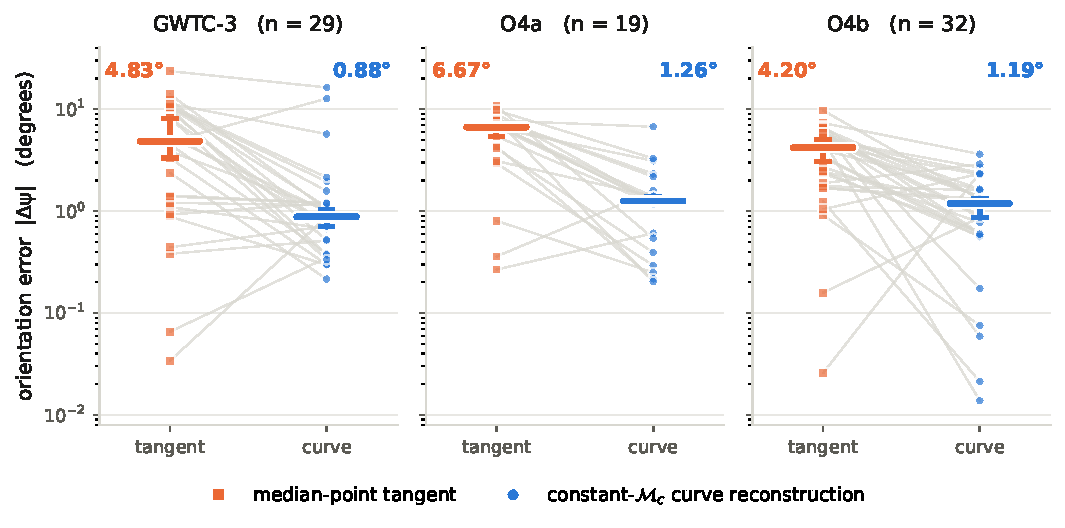
\includegraphics[width=\textwidth]{../figures/fig1b_tangent_vs_curve_residual.pdf}
\caption{\figonebcaption}
\label{fig:1b}
\end{figure}

\begin{figure}[t]
\centering
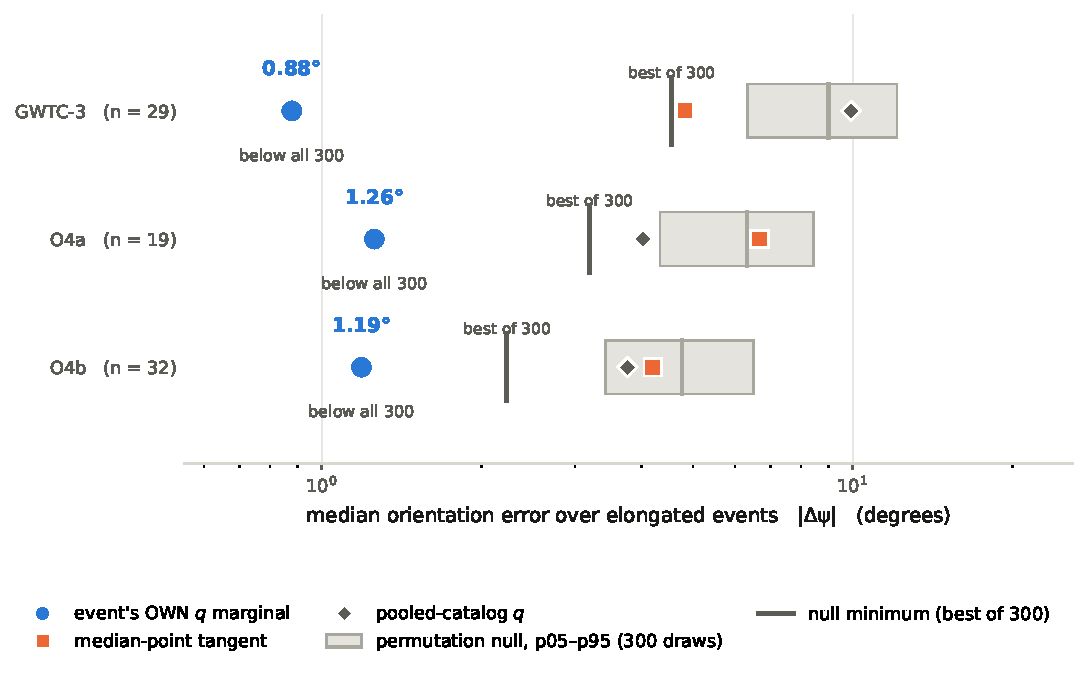
\includegraphics[width=0.92\textwidth]{../figures/fig1c_nontriviality_q_baselines.pdf}
\caption{\figoneccaption}
\label{fig:1c}
\end{figure}

Figure~\ref{fig:1b} shows the per-event comparison behind the table: every elongated event is drawn as a
line from its tangent error to its curve error, so the reader sees the whole distribution rather than a
summary.

\subsection{The reconstruction is not trivial}
\label{sec:nontrivial}
A curve fitting a curved posterior better than a straight line is unsurprising. The substantive question is
whether the \emph{event's own} $q$ marginal matters, or whether any plausible marginal would do. It matters
(Fig.~\ref{fig:1c}). Replacing it with a marginal pooled over the catalog, or with another event's, degrades
the median error by $2.5$--$12\times$; and the achieved error lies below the \emph{minimum} of $300$
catalog-stratified permutations in each catalog, so the permutation $p$-value is $<1/300$ throughout. We
report the permutation distribution rather than a single shuffled assignment: one draw is not a null, and
re-drawing it moved the O4a figure from $3.04^\circ$ to $8.62^\circ$.

A sharper check addresses the circularity concern directly. Using waveform family A's median chirp mass and
$q$ marginal to reconstruct family B's \emph{separately inferred} principal axis --- never touching B's own
geometry --- gives $2.08^\circ$ (A$\to$B) and $2.78^\circ$ (B$\to$A) over $64$ events elongated in both,
against a $1.99^\circ$ reference scale set by how far the two families' measured axes sit from each other.
The reconstruction therefore transfers between independent inferences of the same event and is not an
artifact of reusing one posterior's Monte Carlo noise. We call $1.99^\circ$ a reference scale, not an error
floor: a reconstruction could in principle denoise a posterior functional and beat the raw A--B
disagreement.

\section{Why the geometry is structured}
The structure is expected. The inspiral phase is dominated at leading (0PN) order by $\mathcal{M}_c$, so the
Fisher information has one sharply-measured (``stiff'') direction --- constant $\mathcal{M}_c$ --- and
poorly-measured (``sloppy'') directions transverse to it \citep{Transtrum2015}, and the posterior's long
axis therefore lies along the constant-$\mathcal{M}_c$ level set. The distinction between the tangent and
the curve is the distinction between linear principal-component analysis and a \emph{principal curve}
\citep{HastieStuetzle1989}: the principal axis of samples spread along a curved arc is a chord, which is
rotated off the tangent at the median point.

We can do better than invoke that framework by name. \citet{HastieStuetzle1989} define a principal curve by
\emph{self-consistency}: $f(t)=\mathbb{E}[X \mid t_f(X)=t]$, i.e.\ every point of the curve is the mean of
the data projecting onto it. This is directly testable for the constant-$\mathcal{M}_c$ curve, and it
fails: projecting each posterior sample to its nearest curve point and comparing that point to the mean of
what lands there leaves a perpendicular offset of about 3.1\% of the posterior's own scale. The
constant-$\mathcal{M}_c$ curve is therefore \emph{not} a principal curve of the posterior --- and the size
of that failure is what predicts the reconstruction residual (Sec.~\ref{sec:residual}).

We deliberately do not dress this in stronger language than the analysis supports. We compute no
Fisher--Rao quantity, and the measured object --- the principal-axis angle of a sample covariance in fixed
$(m_1,m_2)$ coordinates --- is not invariant under reparameterization; it changes under a change of mass
coordinates, and we state the convention rather than implying invariance. Sec.~\ref{sec:frames} reports the
frame and coordinate dependence explicitly. The closest published neighbours stop short of this measurement in
identifiable ways. \citet{Hannam2013} state that ``the component masses consistent with the signal lie
roughly along a line of constant chirp mass'' and label chirp mass on their confidence regions, but make no
quantitative statement about posterior orientation. \citet{Ohme2013} apply principal component analysis to
the post-Newtonian phase coefficients rather than to $(m_1,m_2)$ posterior samples, predict no per-event
orientation, and validate against no catalog. The \texttt{simple-pe} metric of \citet{Fairhurst2023}
assumes the match ``varies quadratically with the difference in parameters'' about a peak, yielding an
error ellipse --- the same local, linear class of approximation as our tangent term, though computed in
$(\mathcal{M},\eta)$ rather than $(m_1,m_2)$ coordinates --- and those authors themselves note they
``observe curved contours rather than perfect ellipses''. To our knowledge no published work reconstructs
the per-event $(m_1,m_2)$ posterior orientation from the chirp-mass curve over the event's own $q$
marginal, or validates such a reconstruction out-of-sample across catalogs; that application is the
contribution here.

\section{The residual is a real systematic}
\label{sec:residual}
The $\sim\!1^\circ$ residual is not sampling noise. Bootstrapping the released posterior samples --- drawing
one index set and recomputing \emph{both} the measured axis and the curve inputs from it, so their
correlated Monte Carlo errors cancel --- gives a median resolution of $0.19^\circ$ on the difference,
against a median discrepancy of $1.03^\circ$: a ratio of about six. The constant-$\mathcal{M}_c$ curve is
an excellent but imperfect description of posterior orientation, and the gap is a property of the model,
not of the sample count.

We are careful about what this bootstrap measures. It is the \emph{Monte Carlo resolution} of the released
sample set: it shrinks as more samples are released and encodes nothing about detector noise, calibration,
waveform systematics or population variation. It is therefore not coverage, and we do not quote the
fractions of events falling within one or two bootstrap widths as though they were.

The residual carries a signed component --- the curve under-rotates relative to the measured axis by a
median $0.78^\circ$ --- but this is not uniform across catalogs: it is significant in the training catalog
($p<0.001$) and in O4a ($p=0.019$), and \emph{not} significant in the newest and largest catalog, O4b
($p=0.38$). We report it per catalog for that reason.

The residual has a mathematical explanation. The per-event self-consistency violation defined above
correlates strongly with the per-event orientation residual: Spearman $\rho=0.68$ ($p=5e-12$) at our primary
projection grid, and $\rho$ between $0.64$ and $0.68$ across a sweep of grid resolutions, so the result
does not rest on that tuning choice. This is a correlation between two independently measured quantities
rather than a fit, so it cannot be inflated by added model freedom. Replacing the curve by those
conditional means --- one Hastie--Stuetzle iteration --- reduces the residual in-sample, but we do not
claim it as an improved reconstruction: the improvement is grid-sensitive (median $0.35$--$1.08^\circ$
across the sweep), and in a cross-waveform-family test it improves in both directions but reaches
$p<0.05$ in only one ($1.14^\circ\!\to\!0.66^\circ$, $p=0.024$; $1.00^\circ\!\to\!0.69^\circ$, $p=0.064$).

A second mechanism is supported. The curve model has zero thickness, whereas a real posterior has finite width
perpendicular to the curve --- a median of about a third of its total spread. Learning that width profile on
one waveform family and using it to reconstruct another family's axis improves on the zero-thickness curve
in both directions ($1.14^\circ\!\to\!0.96^\circ$, $p=0.005$; $1.00^\circ\!\to\!0.74^\circ$, $p=0.028$), so
finite thickness is a genuine out-of-sample contributor. The \emph{arc-varying} part is not established: a
constant thickness performs as well as the measured profile in one direction, and simple linear or
quadratic tapers match or beat it in both. We therefore attribute no specific fraction of the residual to
the measured taper.

\section{Frames, coordinates, and the elongation gate}
\label{sec:frames}
The measured object is a Euclidean principal-axis angle in fixed coordinates and is not
reparameterization-invariant; we therefore state its dependence rather than assume it away. Repeating the
primary score in \emph{detector-frame} masses gives $0.31^\circ$ against $1.03^\circ$ in the source frame
(paired over the same $81$ events, $p=4\times10^{-9}$), and in $(\log m_1,\log m_2)$ gives $0.77^\circ$.
The detector-frame gain is largely \emph{mediated by elongation}: removing the redshift uncertainty that
source-frame masses import makes posteriors markedly more elongated (median axis ratio $9.9$ versus $4.6$),
and at matched axis ratio the two frames perform comparably --- the detector frame is in fact worse in the
$3$--$5$ band. We therefore say the difference is consistent with mediation by elongation, not that the
detector frame suits the model better. The source frame remains the locked primary score; the
detector-frame analysis is post-hoc. In $(\mathcal{M}_c,q)$ coordinates the construction is degenerate by
design: a constant-$\mathcal{M}_c$ curve is a vertical line, so the reconstruction carries no per-event
content there.

The restriction to elongated posteriors is physical, not a tuning knob. As the covariance approaches
isotropy the principal axis ceases to exist, and the score degrades smoothly toward the random baseline:
median error $14.5^\circ$ for $\mathrm{axr}\in[1,1.5)$, $7.2^\circ$, $6.0^\circ$, $1.4^\circ$ and
$0.6^\circ$ for successive bands. Nothing distinguishes the chosen threshold of $3$: the curve error falls
monotonically and smoothly across thresholds from $1.5$ to $10$.

\begin{figure}[t]
\centering
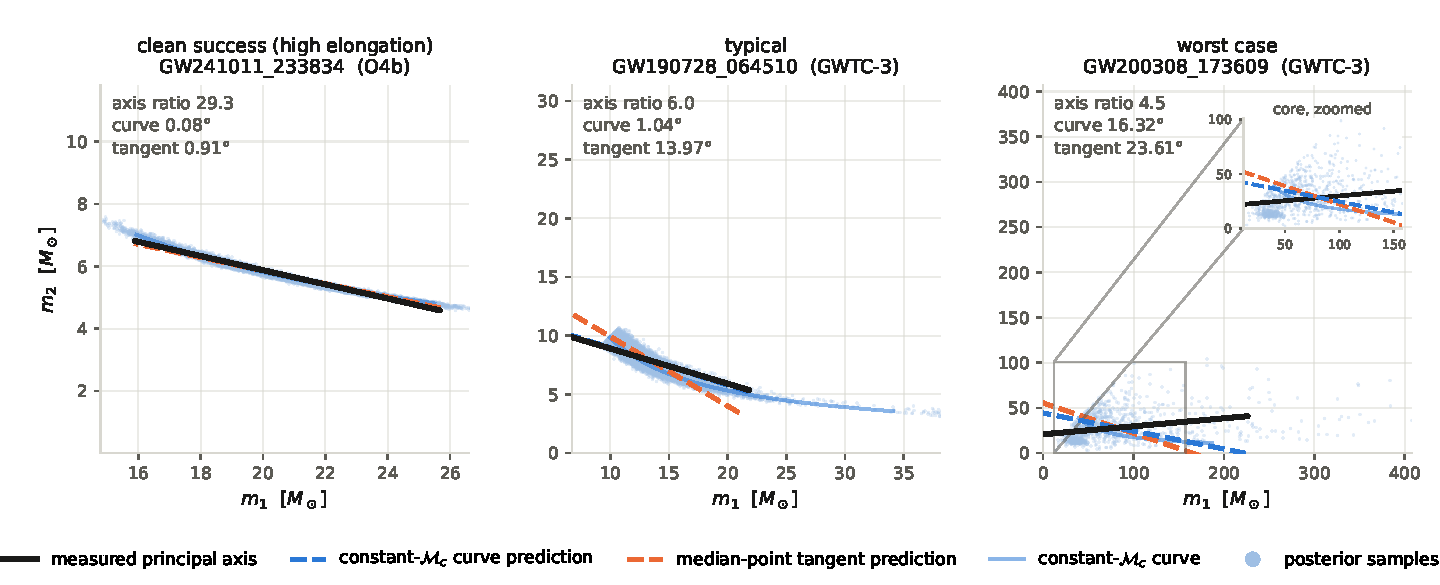
\includegraphics[width=\textwidth]{../figures/fig2a_posterior_geometry_examples.pdf}
\caption{\figtwoacaption}
\label{fig:2a}
\end{figure}

Figure~\ref{fig:2a} shows what the numbers describe, for three events chosen by stated rules including the
worst case in the sample.

\section{Coherence as a systematics detector}
If the geometry is measurement optics, then \emph{departures} from it are informative, and departures that
are \emph{coherent} across events are systematics rather than physics. We test this in two ways. First, a
physics-blind ``outlier atlas'': ranking the elongated O4b events by their curve residual and correlating
against nine pre-declared axes (precession $\chi_p$, aligned spin $\chi_{\rm eff}$, mass ratio, redshift,
signal-to-noise ratio, chirp mass, total mass, secondary mass, and waveform-family disagreement) with
Benjamini--Hochberg control and a partial correlation removing the axis-ratio confound, \emph{no physical
axis} survives; the only surviving correlate is waveform-model disagreement --- a measurement systematic,
with a sign indicating that the curve tracks the waveform \emph{ensemble} consensus better than any single
waveform tracks another. Second, and more sharply, the geometric exponent fit of
Section~\ref{sec:gr} exhibits a coherent $3\sigma$ ``deviation'' that the same lens correctly identifies as
a systematic. The methodological rule --- an anomaly coherent across independent datasets is a systematic,
not a signal --- is thus both stated and exercised.

\section{An exploratory geometric diagnostic --- and why it is not a test of GR}
\label{sec:gr}
The exponents of $\mathcal{M}_c$ are fixed by the 0PN quadrupole formula. Generalize to the one-parameter
family
\begin{equation}
\mathcal{M}_p = (m_1 m_2)^p (m_1+m_2)^{1-2p}, \qquad \text{GR: } p = 3/5 = 0.600,
\end{equation}
and fit $p$ to the posterior orientations: because orientation is scale-free
($m_1(q;p)\propto q^{-p}(1+q)^{2p-1}$), the fit isolates the exponent from the mass scale.

\textbf{This is not a test of general relativity, and we do not present it as one.} The posterior samples
were themselves produced with general-relativistic waveform models; fitting an effective exponent to their
geometry probes the internal consistency of those inferences, not the theory that generated them. No bound
on modified inspiral phasing follows. We retain the exercise only because it is a sensitive diagnostic of
the reconstruction's own imperfections. On the O4b elongated events alone we find
$p = 0.616\pm0.011$; combining O4a and O4b, $p = 0.628\pm0.009$.

Taken naively this is a coherent $3.1\sigma$ departure from GR --- and it is a false alarm. Two
pre-committed checks demote it. (i) The two disjoint event catalogs disagree with each other by $0.031$, as
large as the offset from GR ($0.028$); this catalog-to-catalog spread is a systematic that the
bootstrap statistical error ($0.009$) does not capture. Including it, $p = 0.628\pm0.009\,(\mathrm{stat})\pm
0.016\,(\mathrm{syst})$, or $1.5\sigma$ from GR. (ii) The per-event exponent depends on elongation
(Spearman $= -0.41$, coherent in both catalogs); the cleanest, most-elongated half yields $p=0.606$,
consistent with the GR value. The offset is therefore a finite-width imperfection of the leading-order
geometric model, coherent across catalogs, and vanishing in the clean limit. It is a diagnostic of the
model, not a measurement of gravity, and it belongs in an appendix rather than in the headline claims.

\section{The information anatomy of a detection}
The same Fisher structure that fixes the posterior orientation also fixes \emph{when}, in frequency, each
parameter's information arrives. Computing the cumulative Fisher information for the chirp mass (0PN), mass
ratio (1PN) and spin (1.5PN) across all $190$ real O4a+O4b events, the ordering $\mathcal{M}_c<\eta<\chi$
holds universally: the chirp mass is always determined earliest ($\sim35$~Hz), spin latest, and the
frequency separation --- the anatomy's ``richness'' --- is a monotonic function of total mass (Spearman
$-1.00$), widest for light, long-inspiral systems and compressed for heavy ones that merge immediately in
band. This is a frequency-resolved, per-event map of what each detection measured and when. It is a forward
prediction from the waveform model; a fully data-driven version (re-analysing loud events in frequency
slices and comparing empirical to GR-predicted information accumulation) is left to future work.

\section{The loudest event: GW250114}
As an application, GW250114 --- the loudest event to date (network SNR $\sim80$), a near-equal-mass binary
black hole with remnant $M_f^{\rm src}\approx62.7\,M_\odot$, $\chi_f\approx0.68$ --- is essentially a much
louder counterpart of the first detection GW150914. Its remnant predicts Kerr quasi-normal-mode frequencies
of $248.9$~Hz ($\tau=4.10$~ms) for the fundamental and $243.4$~Hz ($\tau=1.35$~ms) for the first overtone;
a published ringdown analysis using an orthonormal-mode basis reports the first overtone at $99.9\%$
significance --- up from $82.5\%$ in nonorthogonal analyses of the same event --- and finds ``no significant
deviation'' from the Kerr prediction \citep{Suzuki2026}. We quote the orthonormal figure with that context
because the significance is a property of the analysis basis, and we describe the Kerr result as a null,
which is what is reported, rather than as a confirmation of the no-hair theorem. Being
near-equal-mass, its posterior is nearly round and it is (by construction) outside the elongated set used
for the curved law --- an illustration that the loudest events are not always the most informative for a
given geometric probe.

\section{Discussion}
We have shown that the orientation of a compact-binary mass posterior can be reconstructed from two
one-dimensional summaries of that posterior --- its median chirp mass and its mass-ratio marginal --- to
about a degree on elongated events, with no coefficient calibrated on the validation catalogs, and that the
reconstruction holds out-of-sample on two later, disjoint event catalogs. The result is not the trivial
observation that a curve beats a line: substituting another event's marginal degrades it several-fold and
the achieved error lies below the minimum of $300$ permutations, while the reconstruction transfers between
separately inferred waveform-family posteriors of the same event. Its residual is a genuine systematic
about six times the Monte Carlo resolution of the released samples, to which finite posterior thickness is
an out-of-sample contributor. We offer the result as a posterior-compression law and a systematics
diagnostic.

\paragraph{Status of the claims.} Because several of these statements were narrowed in the course of an
internal submission-gate audit, we state their status plainly. The reconstruction, its baselines, its
cross-waveform transfer, its frame dependence and its per-waveform-family stability are reproducible from
committed artifacts. The residual analysis is a Monte Carlo resolution statement, not coverage. The
companion precision law relating chirp-mass fractional width to signal-to-noise and mass is
\emph{exploratory and not established}: its pooled fit rejects the leading-order mass exponent, and the
agreement that appears in a light-mass subset rests on a split chosen after seeing that rejection, so we do
not claim it. The two out-of-sample scores are also not equivalent evidence: the O4b preregistration is
timestamped in the public record before the data were opened, whereas the O4a preregistration entered our
public repository in the same commit as its results and is attested only by a private history. Finally,
O4a and O4b are \emph{disjoint event catalogs}, not independent experiments: they share detectors,
calibration, waveform families, priors and analysis conventions. A separate Bayesian ringdown analysis
performed during this program was retracted after its posterior was found to be prior-dominated; it is
recorded in the project history and forms no part of the results here.

\paragraph{Reproducibility.} The figures in this paper are generated from committed machine-readable
artifacts, and their captions are emitted from the same artifacts so that text and figure cannot drift
apart. Raw parameter-estimation files are not distributed with the code; they are public and are listed
with record numbers in the accompanying data-availability documentation. Analyses read a single cached
extract of those files, regenerated in about five minutes by \texttt{src/e94\_build\_posterior\_cache.py}
once the releases are present; no analysis or figure module reads the raw files directly.

\paragraph{Honest limitations.} (1) This is a posterior-compression result: the $q$ marginal is taken from
the posterior being reconstructed, so it is not a prediction from source medians or external physics.
(2) It is validated on elongated events; round posteriors have no well-defined orientation and are excluded
by design, and \citet{Baird2013} note that constant chirp mass ceases to characterise the mass degeneracy so
cleanly at higher masses, bounding where such a construction should be expected to work. (3) The $\sim\!1^\circ$ residual is explained in the principal-curve sense --- its size tracks the
curve's failure of self-consistency --- but the corresponding one-step correction is not established
out-of-sample, and the arc-varying form of the thickness contribution is not established either. (4) The measured angle is coordinate- and
frame-dependent, and we make no invariance claim. (5) The exponent fit of Sec.~\ref{sec:gr} is a diagnostic
of GR-generated posteriors and cannot bound deviations from GR. (6) The information anatomy is
model-predicted, not strain-extracted. (7) A first-principles derivation of the curve's width and curvature
from the Fisher information remains open. (8) Waveform-model choice contributes a per-event orientation
scatter of a few degrees, the dominant per-event systematic.

\paragraph{Data availability.} All data are public: GWTC-4.0 PE (Zenodo 16053484) and GWTC-5.0 PE (Zenodo
20276106, 20348006). Analysis code, locked pre-registrations, per-event results, and a reproducibility
notebook accompany this work.

\begin{thebibliography}{99}
\bibitem[Cutler \& Flanagan(1994)]{CutlerFlanagan1994} C.~Cutler and {\'E}.~{\'E}.~Flanagan,
\emph{Phys.\ Rev.\ D} \textbf{49}, 2658 (1994).
\bibitem[Poisson \& Will(1995)]{PoissonWill1995} E.~Poisson and C.~M.~Will,
\emph{Phys.\ Rev.\ D} \textbf{52}, 848 (1995).
\bibitem[Baird et al.(2013)]{Baird2013} E.~Baird, S.~Fairhurst, M.~Hannam, and P.~Murphy,
\emph{Phys.\ Rev.\ D} \textbf{87}, 024035 (2013).
\bibitem[Hannam et al.(2013)]{Hannam2013} M.~Hannam, D.~A.~Brown, S.~Fairhurst, C.~L.~Fryer, and
I.~W.~Harry, \emph{Astrophys.\ J.\ Lett.} \textbf{766}, L14 (2013).
\bibitem[Ohme et al.(2013)]{Ohme2013} F.~Ohme, A.~B.~Nielsen, D.~Keppel, and A.~Lundgren,
\emph{Phys.\ Rev.\ D} \textbf{88}, 042002 (2013).
\bibitem[Fairhurst et al.(2023)]{Fairhurst2023} S.~Fairhurst, C.~Hoy, R.~Green, C.~Mills, and
S.~A.~Usman, \emph{Phys.\ Rev.\ D} \textbf{108}, 082006 (2023).
\bibitem[Transtrum et al.(2015)]{Transtrum2015} M.~K.~Transtrum et al.,
\emph{J.\ Chem.\ Phys.} \textbf{143}, 010901 (2015).
\bibitem[Hastie \& Stuetzle(1989)]{HastieStuetzle1989} T.~Hastie and W.~Stuetzle,
\emph{J.\ Amer.\ Statist.\ Assoc.} \textbf{84}, 502 (1989).
\bibitem[Suzuki et al.(2026)]{Suzuki2026} M.~Suzuki, K.~Kubota, S.~Morisaki, H.~Motohashi, and
D.~Watarai, arXiv:2605.03576 (2026).
\end{thebibliography}

\end{document}
